% Introduction

\chapter{Introduction} % Main chapter title

\label{sec:intro} % For referencing the chapter elsewhere, use \ref{Chapter1} 

\lhead{\emph{Introduction}} % This is for the header on each page - perhaps a shortened title

\section{\emph{Motivation}}

It is astonishing how much we can learn from observing and 
contemplating the Universe. All this knowledge of the Universe
led to a better comprehension of the dynamics of the Universe itself 
and how his components galaxies, interstellar/intergalactic
medium and stars has evolved in time. This theories doesn't have
just an academic impact, society have faced different changes of 
paradigm due to this scientific achievements. And hopefully this
knowledge of nature can help us in the path to a modern 
sustainable society with the conscious of our place and role 
in the Universe.  

Astronomy is unique in the sense that there is only one Universe 
to observe. Due to the expanding nature of the Universe and 
that the speed of light is finite, observations of the farther 
regions of the Universe are also from the youngest stages of the Universe.
This allows to observe the evolution of the Universe during redshift.

There are two techniques to measure the radiation coming from the 
Univserse; photometry and spectroscopy. Photometric observations measures 
the flux astronomical objects in different filters. This allows to derive quantities such as the luminosity and the temperature. While spectroscopic observations would let study in deep detail
the spectra of astronomical objects, in particular the spectra of 
galaxies reveals properties such as: the population of stars in the galaxy, the
redshift, the elements that constitute this objects, the characteristics 
of the insterstellar medium and many more.

In particular the Lyman$\alpha$ emission line is a usefull 
tool to detect star forming galaxies at high redshift, specially 
at $z>2$ which is when the line is shifted to the optical frame. But 
as discussed in X the morphology of the line is substantially affected
by the gas kinematics \& distribution, the interstellar gas (IGM)
 and by the dust. 

Understanding the morphology of the \ly line is a crusial endeavour 
to understand deeply the properties of galaxies at high redshift. To this aim 
computer simulations are extremely usefull, models of this properties 
can be simulated to creat synthetic profiles that can be compared
with the observations. 

This is an important era to study this high redshift galaxies. Computer 
simulations techniques have been imporved and more powerfull facilites are
now aveilable. Also a new generation of telescopes are being constructed,
this telescopes would have the power to observe more deeply in the sky, 
and new high redshift galaxies are going to be discovered. This would 
improved our understanding of the high redshift Universe. 

\section{\emph{Historical Remarks}}

The emission of the \ly line in galaxies was first predicted by 
\citep{PartridgePeebles} in 1967, in their work they suggest that the \ly luminosity
could amount the lumonosity of the galaxies at high redshift, and that 
it could be detected. 

By the same epoch the radiative transfer theory in \ly systems started to be
 studied by \citep{Osterbrock62, Adams72,Harrington73, Neufeld90},
 it can be seen as a difussion process if it is carried out in 
 optically thick medium. It means that \ly photons propagating 
in a medium are difussing in space and in wavelenght from the line center.   
Because of the complexity of the systems this analytical solutions 
can only be carried out with simplifications. 


Almost tree decades later \citep{DjorgovskiThomson92} detected the first \ly emmiter galaxy (LAE), since then hundreds of galaxys has been  
observed at redshifts $z>2$ (citaciones). There is a confirmed LAE at $z=8.6$ by \citep{Lenhert2010} and candidates up to $z\sim12$ by \citep{Brammer12}. 
The \ly line have the potential as a tool to confirm galaxies at the highest 
redsifts. 

Despite all this observational efforts to fully understanding radiative
tranfer (RT) of the \ly line numerical simulations started to be performed.
({\bf{citaciones}})

More recently various teams \citep{Mas-Hesse09,LARS} have
observed nearby galaxies with the Hubble Space Telescope. With the
aim to have good resolution spectra and images of the HI distribution 
and kinematics. This new spectra now can be compared with the numerical 
models developed.

 

\section{\emph{The Lyman $\alpha$ line in astronomy}}\label{sec:lyuses}

The Lyman $\alpha$ (Here after \ly) emission line is a consecuence of the 
transition 
from the first excited level to the ground level of the electrons
in the Hydrogen atom. When the electron undergoes in such transition 
a photon is emitted with an energy of $13.6eV$ which corresponds to 
a rest wavelenght of $1215.67 \AA$. 

This transition is very common in the Universe due to the high abundance
of hydrogen. Two main mechanisms end up in \ly radiations: Recombination 
processes and collisional events of Hydrogen atoms. UV stellar radiation
from star regions (Recombination) , Gravitational 
cooling (Collisional) and UV background radiation (Recombination) the interested
reader could be interestes in\citep{LaursenPhD} and references within for
more details. 

The detection of the \ly line has been broadly studied and has multiple 
applications in extragalactic astronomy:

\begin{itemize}
\item {\bf{Detection of high $z$ galaxies:}} One of the most used 
methods to detect high redshift galaxies is finding the \ly emission 
line using Narrow band imaging or Spectroscopy, with this method 
hundreds of galaxies has been detected. This 
allows to study properties of the high redshift Universe such as
the Large Scale structure. 
 
\item {\bf{Galaxy formation and evolution:}} Observed LAEs at different
reshifts have allowed to derive the Lumimosity Functions (LFs) of LAEs, 
for this aim a good knowledge of the escape fracition of 
photons is requiered $f_{esc}$ see \S \ref{sec:fesc} for details on the \ly
photons escape fraction. Understanding the observed LAEs LFs enhance a
better understanding of the galaxy formation models. 

\item {\bf{Reionization:}} The Epoch of Reionization (EoR) is a mayor
epoch in the Universe, in which the neutral cold HI gas reionize to 
become a hot gas. There are evindece from CMB measurements that 
the EoR must start around $z >> 11$ and should end at $z\sim5$. During this 
epoch the intergalactic medium (IGM) became opaque to \ly radiation 
outcomming from high redfshift galaxies. LAEs have shown to be 
very usefull in constrainig the time at wich the EoR ends. For a complete
recent review please see \citep{review}
 
\end{itemize}


\section{Units, Quantities \& Definitions}

Through this work we will use some units and quantities that perhaps the reader
may not be familiar with. Here we define this quantities.

\subsection{Optical depth and Column Density}

The optical depth $\tau$ is a measure of the "transparency" of the medium
in which the photons are propagating. And is defined as:

\begin{equation}
d\tau = \alpha dr
\end{equation}

Where $\alpha$ is the absortion coefficient and is defined as the  :

\begin{equation}
\dfrac{dI}{dr} = -\alpha I
\end{equation}

From this definitions we can now define the "thickness" of the medium,
if $\tau > 1$ we said the medium in optically thick and this means
that a photon with frequency $\nu$ cannot go through without been
absorbed. If $\tau < 1$ the medium is optically thin and the photon
could be pass through with out been absorbed.

The optical depth is  a measure of the distance of the source
of photons to the surface of the medium. It is also very common 
to express the amount of gas between the \ly source and the surface
in of the Hydrogen column density 
$N_{HI}$ which is related with the optical depth by $N_{HI} = \tau/\sigma$
where $\sigma$ is the Hydrogen atom cross section. 

\subsection{\ly line profile units}

The frequency $\nu_{\alpha}$ of a \ly photon in rest frame is
$2.46\times 10^{15}Hz$,
there are two main units in which the frequency of the \ly alpha photons
may be presented in the literature.

The first is a dimensionless vairable $x$ defined as:
\begin{equation}\label{eq:x}
x   \equiv \dfrac{(\nu -\nu_{\alpha})}{\Delta \nu_D}
\end{equation}

Where $\nu$ is the frecuency in the observer frame,
$\nu_D$ is the broadening of the line due to the termal
velocity of the Hydrogen atoms $v_{th}$. Which can be derived
assumming that the Hydrogen gas is in thermal equilibrium
and follow a Maxwellian distribution.

\begin{equation}
\dfrac{m_H v_{th}}{2} = K_B T 
\end{equation}

Where $m_H$ is the Hydrogen atom mass, $K_B$ the Boltzmann constant and $T$
the temparature, the expresion for $v_{th}$ is then:

\begin{equation}
v_{th} = \sqrt{\dfrac{2 K_B T}{m_H}} = 128.5 T^{1/2}\dfrac{m}{s}
\end{equation}

The Doppler shift due to $v_{th}$ would be:

\begin{equation}
\nu'= (1 - \dfrac{\vec{v_{th}}\cdot\vec{n}}{c})\nu_{\alpha}
\end{equation}

Which can be expressed in terms of $\Delta \nu_D$ as:

\begin{equation}
\nu_{\alpha} - \nu' = \Delta\nu_D =  \dfrac{\vec{v_{th}}\cdot\vec{n}}{c}
\end{equation}

It is also common to express the line profile in terms of the velocity $V$
making use of Eq.\ref{eq:x}:

\begin{equation}
V = xv_{th} = \dfrac{\nu - \nu_{alpha}}c
\end{equation}

\subsection{Average number of scatterings $N_{scatt}$}

The path of a \ly photon inside an {\bf{optically thick}}
HI medium is resonant this is explained in more detail 
in \S \ref{sec:resonant}. It basically means the the \ly photon
after been emitted by the source is absorved by an H atom
and re-emiited in a time scale of $\sim 10^{-9}$ s.
For this reason this process is commonly refered as
a scattering process. The total number of scatterings
is denoted as $N_{scatt}$ and it is proportional to
$\tau^2$.



\subsection{Resonant scattering}\label{sec:resonant}

Hydrogen is the most abundant element in the Universe furthermore
the Lyman$\alpha$ line is a very common line. However the transmission of this
Lyman$\alpha$ photons through the Hydrogen clouds it's not trivial. There 
are two main aspects that heavily influce the morphology of the line.\\

Imagine that  there is one Hydrogen atom which emits 
a \ly photon in the middle of a cloud of Hydrogen atoms which are in the
ground state. The \ly photon will be abosrved and re-emitted from 
the Hydrogen atoms. This process will end up in a random walk in the space,
and the photon can escape the cloud at any point in the surface of it.\\

\begin{figure}[H]\label{fig:rw}
\begin{center}
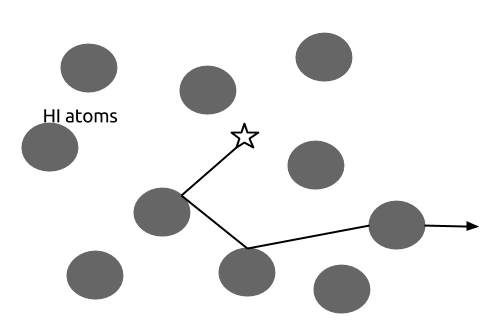
\includegraphics[scale=0.4]{../Figures/randomwalk.png}
\end{center}\caption{Scattering scheme of a \ly photon in a HI medium
(The star is a \ly source and the solid line represents the path that
the \ly photon follow before scaping the cloud).}
\end{figure}


In the previous situation all the Hydrogen atoms were in rest, if the atoms
present proper motions there would be a doppler shift. If an atom have a velocity 
$v$ an emit a \ly photon in the direction opposite to the movement the \ly photon 
would be redshifted. But if it is emitted in the same direcion of movement the
\ly photon would be blueshifted.    

\begin{figure}[H]\label{fig:xshift}
\begin{center}
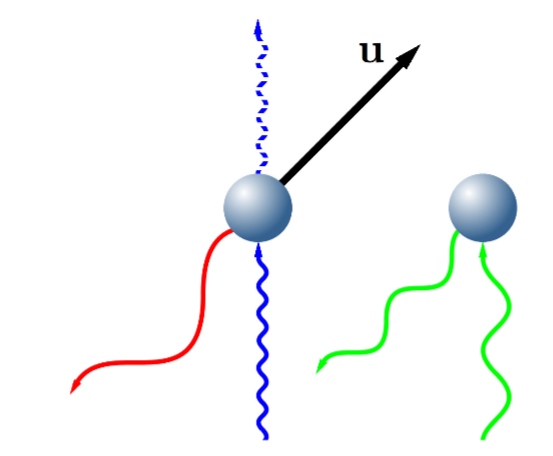
\includegraphics[scale=0.4]{../Figures/xshift.png}
\end{center}\caption{Scheme of the frequency shift. Left: Rest frame, Because 
of the velocity $u$ of the atom absorb a blue-shifted \ly photon, and emmit 
a red-shifted \ly photon. Right HI atom rest frame when all photons have the \ly frequency. (Image credit: Interpereting Lyman $\alpha$ radiation from young, dusty galaxies. By: Peter Laursen, 2010.).}
\end{figure}


This two effects made ratiave trasnfer inside optically thick medium as a random 
walk in space and frequancy. This is why Monte-Carlo methods can be
applyed to this difussion process.
 
\subsection{Escape fraction}\label{sec:ef}

Dust grains are mainly considered as metals in the ISM, these
metals are formed in stars. At high redshifts where galaxies and 
stars are young the most probable escenario in that supernovae 
enrich the ISM with dust \citep{Kotak09}, in this way the observed 
dust \citep{Coppin09}  at high redshift is explained. 

The effect of dust in the \ly transfer inside the ISM is that 
dust grains can absorb (destroy) or scatter \ly photons. The 
probability of this events is given by the 'albedo' $A$ defined as:

\begin{equation}
A = \dfrac{\sigma_{scatt}}{\sigma_{dust}}
\end{equation}

Where $\sigma_{scatt}$ is the total cross section for scattering 
and $\sigma_{dust}$ for absorption. $\sigma_{dust}$ can be derived from 
dust properties see \citep{Laursen09}. 

There are two approaches to the modelling of dust in the \ly RT process.
When the dust distribution is taken as homogeneous in the HI region and 
the \ly photons can be absorbed by the dust or scattered. Or in a clumpy
medium of dust in which \ly photons are more likely to scatter with the 
clumps rather than absorved \citep{Laursen13}. To quantify the effect of 
dust the ratio
of \ly photons observed (\ly alpha photons who manage to scape from the medium) 
over the \ly photons emmited  define the {\bf{escape fraction}} $f_{esc}$. 

It is worth pointing out that the analytical
description of the \ly RT doesn't take into account the precense of
dust. That is a motivation to includ dust in the numerical simulations.
As is explained in more detail in \S \ref{sec:analytic}.  





\section{\emph{ Attenuation of the \ly emission line}}

Despite the fact that the \ly line is the strongest emission line in 
the UV, there were 25 years since the prediction of the \ly line to 
the first observation by \citep{DjorgovskiThompson92}. 
This long absence of the \ly line is what makes this and excited and 
challenging field.

Figure\ref{fig:IGM} shows the outcomming spectra from a galaxy 
at $z \sim 3.5$, the line is double paked as expected from 
the radiative transfer process in the galaxy. After the encounter
with the inter galactic medium (IGM) de blue peak is diminished.
This is beacuse of the expansion of the Universe the blue peak 
is shifted to the \ly frequecy and the HI in the IGM would absorb
part of this radiation. As a result the observed spectra (right figure)
is asymmetric.   

\begin{figure}[H]\label{fig:IGM}
\begin{center}
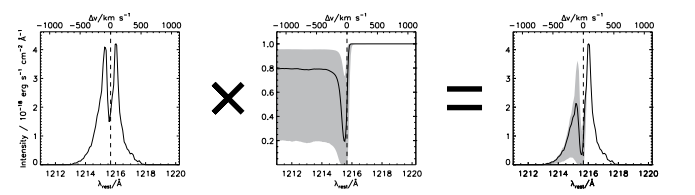
\includegraphics[scale=0.6]{../Figures/ISM.png}
\end{center}\caption{The IGM effect on the \ly line}
\end{figure}


The gas kinematics in the galaxy also plays a mayor role in shaping
the morphology of the line, due to the resonant nature of the line. 
Figure\ref{fig:kulas} show the \ly line
profile for different galaxies at $z \sim 2 - 3$, due to the different
kinematics of those galaxies all the spectra reveals asymmtric profiles 
and some of them are multi-peaked.    


\begin{figure}[H]\label{fig:kulas}
\begin{center}
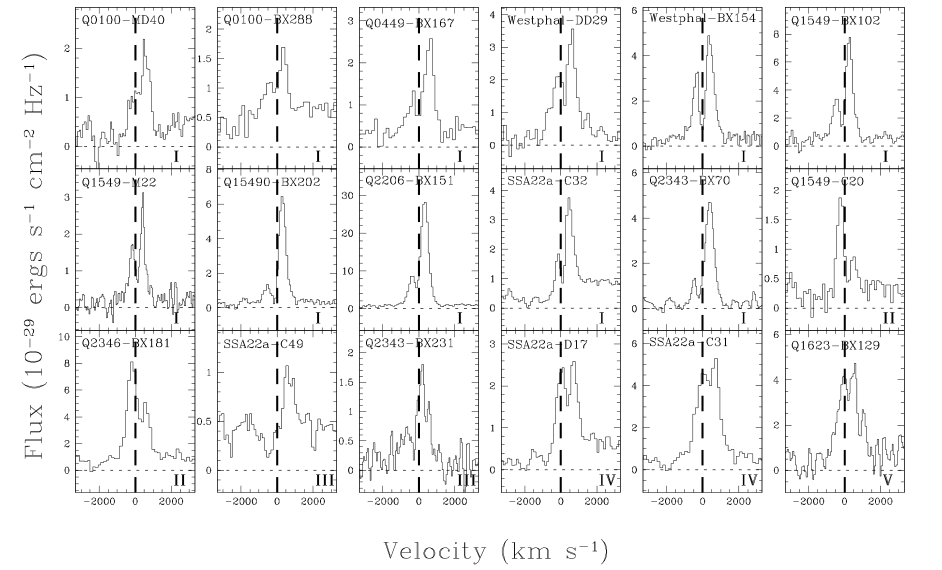
\includegraphics[scale=0.4]{../Figures/kulas.png}
\end{center}\caption{Asymmetry and multipeaked \ly line profiles. (Image credit: The kinematics of multiple-peaked \ly emission in star-forming galaxies at $z\sim 2$ - 3. Kulas, K. et al 2011) }
\end{figure}

The presence of dust in galaxies also play an important role, dust as explained
 in \S\ref{sec:ef} could either absorb or scatter \ly photons. As a 
consecuence dust mainly diminuish the intensity of the \ly line of LAEs. 

Alongside these processes when observing the abundance of LAEs across
the history of the Universe the population of LAEs increases 
with the redshift. But at reshift $z>6$ the  
abundance of LAEs decrease \citep{Schenker12}. Apparently 
 reionization  is governing at that redshift and the IGM medium 
becomes opaque to \ly radiation.   

All this effects makes the \ly line a sensitive line and challenging
to observe at $z>6$ see \citep{Sobral15}, but with valuable information
of the ISM/IGM distribution and kinematics. All This makes de \ly
line a very usefull line to explore the extragalactic Universe as
discussed  in \S\ref{sec:lyuses}.

  

\section{\emph{Analytical Models}}\label{sec:analytic}

Understanding the \ly line profile requieres a theory knowledge
about the physics processes involving the radiatie transfer. Symplified 
situations have been studied in order to obtain an analytical 
 profile. This models provide the theory that
would let develope the modern codes enable to 
This models are the foundations. In this section the most relevant 
analytical models are explained in the chronological in which 
they have been developed. 

The radiave transfer of \ly photons has been studied by several authors
see \citep{RybickiLightman79} for a complete treatment, the Intensity
of \ly photons can be studied via:
 
\begin{equation}\label{eq:RT}
n\cdot\nabla I(\nu, n)= - \alpha_{\nu} I(\nu, n) + j(\nu, n) + \int d\Omega' \int dn' I(\nu', n') R(\nu', \nu, n', n)
\end{equation}

Where $\nu$ is the frequency of the \ly photons. $n$ is the direction 
of the \ly photon. $I(\nu, n)$ is the intensity
of the radiation. $\Omega$ is the solid angle. $R(\nu', \nu, n', n)$ 
is the redistribution function, basically this function which measures 
the probability that a \ly photon with frequency $\nu'$ and direction $n'$
after scatters have a frequency $\nu$ and direction $n$.

The mean density $J_{\nu}$ is defined as:

\begin{equation}\label{eq:J}
J_{\nu} = \dfrac{1}{4\pi}\int I_{\nu}d\Omega
\end{equation}


Using Eq.\ref{eq:J} and following the above steps:

\begin{itemize}
\item In an optically thick medium the dependece on the direcion {\bf{$n$}} can 
be neglected.
\item Using a Taylor expansion in ($I(\nu', n')$) in the second term of the right in Eq.\ref{eq:RT} 
\item Replacing the absorption coefficient in terms of the optical depth.
\item $j(\nu, n)=0$ and $\sigma_{dust}=0$
\end{itemize}

Eq.\ref{eq:RT} can be expressed as: 

\begin{equation}\label{eq:RTeq}
\dfrac{dJ(\nu)}{d\tau} = \dfrac{(\Delta \nu_D)^2}{2}\dfrac{\partial}{\partial \nu}\phi(\nu)\dfrac{\partial J(\nu)}{\partial \nu}
\end{equation}

Where $\phi(\nu)$ is a Voigt profile (Combolution of a Gaussian profile  
and Lorentzian profile), this Voigt profiles respond to the resonant nature 
of the line. Eq.\ref{eq:RTeq} is a diffusion equation in space and frequancy
for the \ly photons in HI clouds. Different authors have solved 
Eq.\ref{eq:RT} in simplified situtations that we are going to discuss above. 

\subsection{Infinite Slab with \ly source at the center:}

The first analyitical solution to the RT Eq.\ref{eq:RTeq}
was an effort in which different authors made a contributions \citep{Unno55, Osterbrock62, Adams72, Harrington73} and ended with the analytical expresion
derived by \citep{eufeld90} based on the previous works. 

\begin{equation}
J(\tau_0, x) = \dfrac{\sqrt{6}}{24}\dfrac{x^2}{\sqrt{\pi}a\tau cosh[\sqrt{\pi^3/54}(x^3-x_{in}3)/a\tau]}
\end{equation}

Where $a$ is the Voigt parameter defined as $a=A/4\pi\Delta \nu_D$. \citep{Harrington73} also show that the maximum intensity of the line is at:

\begin{equation}
x_m = \pm1.066(a\tau)^{1/3}
\end{equation}

And the averge number of scatterings is:

\begin{equation}
N_{scatt} = 1.612\tau
\end{equation}

In Fig.\ref{fig:slab} the analyticial profile of the slab solution is shown, 
the solid line is the simulated profile reproduced with \citep{CLARA} the code
used in this work.

\begin{figure}[H]\label{fig:slab}
\begin{center}
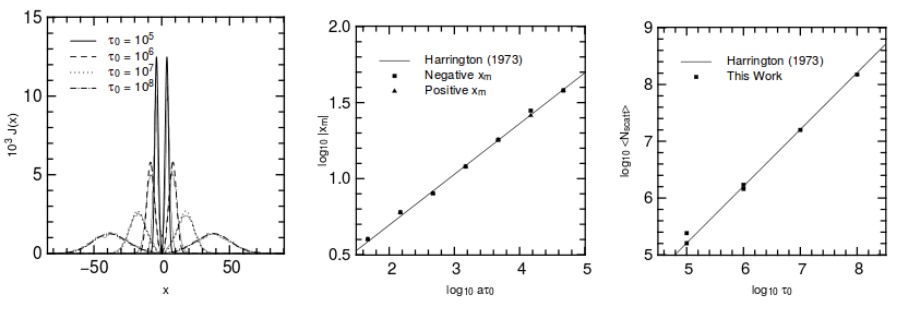
\includegraphics[scale=0.4]{../Figures/slab.png}
\end{center}\caption{(left) Analytic profile for a dustless infinite slab with central
\ly souces. (Middle) Maximum peaks position. (Right) Average number of 
scatterings $N_{scatt}$ in function of the optical depth $\tau$.(Image credit:  CLARA's view on the escape fraction of \ly photons in high redshift galaxies. J.E Forero-Romero, et al 2011)}
\end{figure}

\subsection{Spherical solution}

For a spherical gas dustless distribution with central \ly sources \citep{Dijkstra06} has shown that the emergent spectrum is described by the following expresion:

\begin{equation}
J(\tau_0, x) = \dfrac{\sqrt{\pi}}{4\sqrt{6}}\dfrac{x^2}{a\tau (1+cosh[\sqrt{2\pi^3/27}x^3/a\tau])}
\end{equation}

The analytical spectrum of the spherical solution 
is shwon in Fig.\ref{fig:sphere} for different optical depths. 

\begin{figure}[H]\label{fig:sphere}
\begin{center}
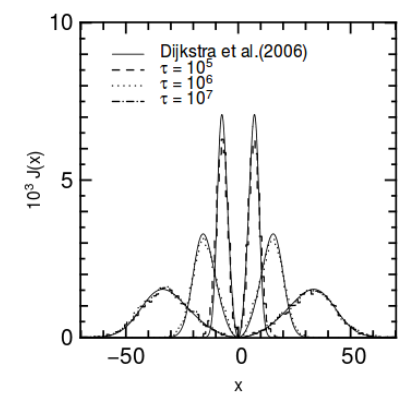
\includegraphics[scale=0.4]{../Figures/Sphere.png}
\end{center}\caption{Analytic profile for a dustless sphere with central \ly sources.  (Image credit: CLARA's view on the escape fraction of \ly photons in high redshift galaxies. J.E Forero-Romero, et al 2011)}
\end{figure}

\subsection{Spherical rotating sphere}

In this work Mark Dijkstra has shown also that an approximate analytical profile
can be derived for a {\bf{rotating spherical distribution}} Eq.\ref{eq:spherero}
with central sources and dustless. This would be the first time that an analytic
al profile is derived for a non-static medium.  

\begin{equation}\label{eq:spherero}
J(x,b,\phi,i)=\frac{\sqrt{\pi}}{\sqrt{24}a\tau_0}\Bigg{(}\frac{(x-x_{\rm
b})^2}{1+{\rm cosh}\Big{[}\sqrt{\frac{2\pi^3}{27}}\frac{|(x
-x_{\rm b})^3|}{a\tau_0}\Big{]}}\Bigg{)}
\end{equation}

\begin{equation}
J(x,i)=2\pi \int_0^Rdb \hs b \int_0^{2\pi}d\phi \hs
S(b,\phi)J(x,b,\phi,i) \approx 2\pi \int_0^Rdb \hs b
\int_0^{2\pi}d\phi \hs J(x,b,\phi,i)\\ \nonumber
\end{equation}

\section{\emph{Simulated models \& techniques}}

In the Universe most of the galaxies have complicated
geometries (Spirals, irregular) and kinematics that 
can not be resolved analiticaly. There are two approaches
to uderstant this complicated properties of galaxies, based
on Monte-Carlo simulations.The first approach is by implementing 
the properties of galaxies in the codes, such as: The geometry
of the gas, the kinematics of the gas and the dust. In this 
approach every property is isolated simulated in order
to compute the \ly profiles, escape fractions, averge number
of scatterings, position of the maximum peaks among others. 

Realistic galaxy properties in the sense of gas geometry
and kinematics using hydrodynamics simulations. In this 
approach the galaxy can be simulated isolated see \citep{Verhamme12}
or galaxies in the cosmic web can also be studied see\citep{Yajima12}.
The temperature, density and gas velocity fields are obtained from 
the hydrodinamic simulations and then the Monte-Carlo code is 
implemented in order to compute the profile properties.

\subsection{Monte-Carlo approach:}

Monte-Carlo (MC) simulations are broadly used in a varierty of 
areas such as science, economy, traffic simulatios among 
many more. MC methods are mostly based in the
generation of random numbers that are the core of 
random walks. This is why MC is used to study the
\ly profile. Here we breafly describe how this method 
work. The main thing is that every every \ly photon is simulated
separately in the following scheme, for a detailed description 
please see chapters $6-8$ in \citep{LaursenPhD} .

\begin{itemize}
\item  The temperature (T) is very common to take $T=10^4K$, gas distribution ($\tau$) and kinematics ($V$) is implemented. 

\item Initialize your \ly photon initial position and frequency $x_{in}$

\item Generate a random displacement ($\tau_0$) of the photon in a random 
direction {\bf{$\vec{n}$}}.

\item  Derive the HI atom velocity components from the initial field, 
and generate random components for the thermal movements.

\item  Set the new direction of the \ly photon after scattering.

\item If the \ly photon encounter a dust particle the albedo probability 
would define if the atom is absorbed or scattered. In also common to take $A=1/2$

\item Repeat from step 2 untill the photon reaches the HI surface at $\tau$.  

\end{itemize}

With this method the final frequency $x_{out}$, the average number of scatterin
gs $N_{scatt}$ can be computed for every step in the random walk.


\subsection{Numerical Models of \ly profiles:}

Using the MC method explained above different RT  codes 
\citep{DijkstraKramer, Laursen09, Verhamme06, CLARA}
have been developed in order to understand the effect of the gas kinematics in
the \lya line, expanding/contracting shell/spherical geometries
has been broadly studied \citep{Ahn03,Verhamme06,Dijkstra06}.
Realistic ISM/IGM medium has also been studied, the effect of a clumpy
medium is discussed in \citep{Hansen06}. Anysotropic \ly emission 
has been studied by \citep{Zheng2013}. And realistic exapanding mediums 
in cavities has been recently studied by  \citep{Behrens2014} 
Hydrodynamic simulations have studied the outcomming spectra of
LAEs in large scale simulations \cite{Forero12}. 
Recently Monte Carlo codes have been used in hydrodynamic 
simulations to study in detail individual galaxies and galaxies 
in the cosmic web.
\citep{Laursen09,Barnes11,Verhamme12,Yajima12}

Figure \ref{fig:out} shows the effect of outflow/inflow kinematics, 
In the ouflow regime photons are blueshifted and the blue part of the line
is stronger than the red part. In the inflow regime the opposite effect
is carried out, the \ly phtons are redshifted. 

\begin{figure}[H]\label{fig:out}
\begin{center}
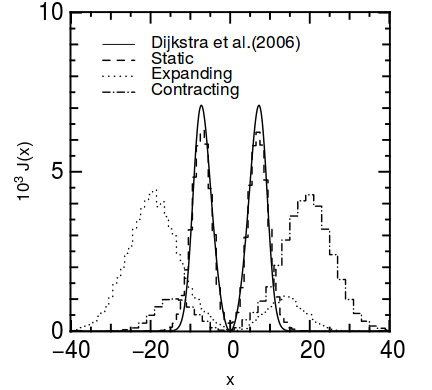
\includegraphics[scale=0.4]{../Figures/out.png}
\end{center}
\end{figure}

\section{\emph{This Thesis}}

In this thesis we study the effect of rotation, an intrinsic
 characteristic of galaxies, on the morphology
of the \lya outcoming profile, to this aim we implement a solid body
rotation model in the radiative transfer code \verb+CLARA+ \citep{CLARA}.
All the codes used for the analysis of this work is reproducible
and public available in \href{https://github.com/jngaravitoc/RotationLyAlpha}{github}.

\subsection{The importance of modelling the effect of gas bulk rotation}

Untill now the effect of rotation have never been studied, and this is 
an intrinsic propertied of all galaxies. In this work we study for the 
first time the effect of galaxy rotation the morphology of the \ly line.

Modelling the effect of rotation in the morphology of the \ly line, push
further our understanding of the effect of the kinematics of the HI regions
on the line. With the knowledge more models into account more 
realistic analysis can be made in observed \ly spectra. 
Now a distinguish between the differents stages of the gas kinematics
 outflow/inflow, anysotropy \ly emission, shell cavities and now
 rotatinal can be made.

Deriving and analytic expression for rotation is also important for
the community, computing an analytic solution is more efficient than
making all the radiative trasnfer simualation. Radiative transfer codes
can be tested against the analytic solution and observed spectra could
be easily fitted  with the model. 

\subsection{Summary of the thesis}

A lot of progress has been done in modelling the \ly line using radiative
trasnfer codes. Properties of the gas kinematics such as outflows/inflows. 
Geometries such as slabs, spheres, cavities and the propagation of \ly photons
in a clumpy media. Dust effects XX. In this thesis we study the effect 
of rotation in the morphology of the \ly profile.  

We model a galaxy as an sphere, with an homogeneous mixture of gas and dust. 
We took the rotation velocity, the optical depth, the viewing angle as free
parameters of the model. We also have two different sources of \ly photons:
A central distribution in the galaxy and an homogeneous distribution. 

We quantify the effect of rotation with the following characteristics: 
Escape fraction of \ly photons, the width of the \ly line, the average number
of scatterings of the \ly photons and with the position of the \ly line maxima.

Our main finding is that rotation do have an important effect on the morphology 
of the \ly line. Specially in the width of the line and in the position of the 
maxima. While the average number of scatterings  and the scape
fraction remain constant.

The line broadens proportional to the rotation velocity, and also the flux in 
the middle of the line increases with rotation.

The axys of rotation breaks the symmetry of the system, Althogh 
observers in different viewing angle with respect to the rotation axys
observe the same amount of flux of the \ly profile. This result
lead us to find an approximate analytic solution to model rotation.
 
 
With these results an approximated analytical solution was derived, 
taking into the account that the radiative transfer inside de gas
cloud is exactly as in the static case. In the sphere surface
a Doppler shift due to the difference velocity of an external 
obsever and the surface have to be taken into account.  


\subsection{Future work}

There are two main projects which are based on the results obtained in 
this work. With the aim of testing our model with observations and
improving the kinematic models of the gas by studying two joint effects
such as outflows and rotation.  

There are LAEs which are governed by rotational movements, also 
have spherical shapes and the main \ly sources are in the center. 
With this propertis such galaxies have the same properties 
that we studied in this work.  
Fitting \ly line profile in order  to meassure the rotational 
velocities of such galaxies would be the direct application 
and test of our model.

Despite the fact that outflows have been broadly studied rotation should 
also be present on this galaxies. The joint effect of the two above properties 
should have a direct effect on the morphology of the \lya line. We are 
 combining the effect of rotation followed by an outflow. For the rotation 
part we are using our analytic solution and for the outflows we are using 
the shell described in \citep{Verhamme06}.

\begin{figure}[H]\label{fig:LARS}
\begin{center}
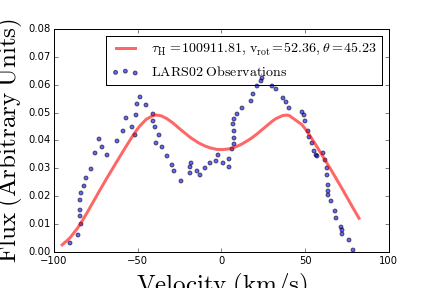
\includegraphics[scale=0.8]{../Figures/LARS02_fit.png}
\end{center}
\end{figure}

